\section{目的}
固体ロケット推進剤を理解するとともに火薬の合成・混合を理解する。
\section{火薬取締法と航空法}
本実験は火薬取締法・航空法[1]を順守して実施している。18歳未満の学生には火薬の調合は行わせておらず、また理化学実験上一回の製造量も既定の範囲内、使用量も法に則って行っている。
 航空法に基づき高度100m以上に到達するロケットは飛ばしていない。
\section{火薬の定義と分類}
火薬とは高温・高圧の化学反応面が伝搬する速度がその爆発物内の音速よりも遅いものである。このような燃焼速度での燃焼状態を爆燃または単に燃焼といい、燃焼面の伝搬速度を燃焼速度という。
 一方、爆薬は高温・高圧の化学反応面の伝搬速度が爆発物内の音速よりも速いもので、非常に急激な燃焼を爆轟という。この場合の爆轟面の伝搬速度が爆速である。
 火薬や爆薬というのは使用されるときの状態を一般的にそう呼ぶのであってどちらも火薬類なのである。
分類としては大きく二つに分けられ化合火薬類、混合火薬類である。前者はペンスリット、ニトログリセリン、TNTであり後者はダイナマイト、カーリット、黒色火薬などがある。[2]

\section{ロケットエンジンの制作}
\subsection{硝酸カリウムの合成}
ロケットエンジンの材料としていろいろな物が使用されるが、安全面と保管の良さから硝酸カリウムが適材である。
 硝酸カリウムの単体購入でも良いが面白くないので今回は以下の方法により生成する。
\begin{eqnarray*}
  \rm{KCl} + \rm{NH}_4\rm{NO}_3 \longrightarrow \rm{KNO}_3+\rm{NH}_4\rm{Cl}
\end{eqnarray*}
\begin{itemize}
\item 材料\\
硝酸アンモニウム(40g)
塩化カリウム(40g)
精製水(100ml)

\item	手順
  \begin{enumerate}
    \item	精製水をビーカーに取る
    \item	硝酸アンモニウムをそこに投入にかき混ぜる
    \item	塩化カリウムを入れまた混ぜる
    \item そのビーカーを湯煎する
    \item ボウルに水を張り、氷を投入しビーカーを冷ます
    \item しばらくすると綺麗な透明の針状結晶が析出する
  \end{enumerate}
\end{itemize}
※早く析出させたい場合は冷蔵庫に入れておけば良い。
 乾燥させるときは新聞紙に広げ2日ほど日にさらすと良いがエタノールで蒸発させた方が早い。
  「減塩」と書かれている商品は大抵塩化カリが使われているがおすすめはしない。純度が低いからである。
生成された硝酸カリウムは結晶状態であるから乾燥したのち、粉砕して適当な容器に保管しておく。
\subsection{推進剤の混合}
先ほど生成した硝酸カリウムと砂糖を混合し、ロケットエンジンをいよいよ制作する。この工程は混合するだけなので非常に簡単である。
 よく目にする混合比が硝酸カリウム65%、砂糖35%である。このままでも良いし、納得できないのであればいろいろと数値を変えて試してやれば良い。
 他にどうすれば良い推進剤が出来るのか。燃焼するときは粒子径が細かければ細かいほど反応は大きくなる。つまり、粒子径が大きければ推進剤としては成り立たないのである。これは走行実験をして明らかである。粒子径が大きいと走行距離は約20m。粒子径が小さければ走行距離はおよそ100mであった。
 したがって、砂糖は粉糖を使うのが良く、生成した硝酸カリウムはよくよくすり潰すことが肝要である。

\subsection{エンジンの組み立て(E-45を例に)}
材料として「内径20mmの塩ビパイプ」、「推進剤」、「径20mm以内の木の棒」、「5.5mmドリルビット」を用意する。
 塩ビパイプを13cmの長さに切り落としておく。木の棒に下図の様にしるしを入れておく。

\begin{figure}[H]
  \centering
  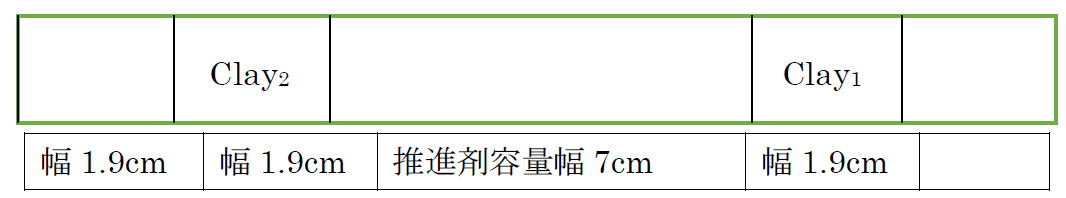
\includegraphics[height=1.5cm,clip]{okada/image/ki.png}
  \caption{木の棒}
  \label{fig:ki}
\end{figure}
この木の棒のメモリにしたがって塩ビパイプの中に推進剤を詰め込んでいく。Clayと書いた幅1.9cmの箇所には砂などを使用すれば良い。
 これに従って詰められたら次は燃焼用の穴をあける。ここでドリルビットを使用する。上に詰めているClay2に穴をあけないように注意する。
 以上でロケットエンジンの完成である。非常に簡単なものだ。[3]
\section{数種の推進剤の混合比表}
\subsection{硝酸カリウムと砂糖、アルミ粉末、硫黄}
推進剤の能力を引き上げる為にアルミやマグネシウムなどの金属粉末がよく使用される。
\begin{table}[H]
\caption{推進剤混合比表}
\centering
\begin{tabular}{c||c|c|c|c}
推進剤材料    &$P_1$ (\%)	&$P_2$ (\%)	&$P_3$ (\%)	&$P_4$ (\%)\\ \hline
硝酸カリウム  &60	         &60	       &60         &50\\
粉砂糖       &20          &10         &10         &10\\
アルミ粉末	  &15	          &20	&25	&25\\
硫黄	&5	&10	&5	&15\\ \hline
\end{tabular}
\end{table}

\subsection{硫黄と亜鉛粉末}
硝酸カリウムと砂糖などの混合推進剤に続いて愛好家の間で知られているのが硫黄と亜鉛粉末の混合による推進剤である。これらの混合による推進剤は大変力強い推進力が得られるが、適切な混合比および適切なノズルを付けなければ力が大きすぎたり、小さすぎたりする。制御が難しいためエンジン試験からは除外した。一般的に硫黄が34\%付近、亜鉛粉末が66\%付近で混合されるようである。
 亜鉛と硫黄の混合火薬については[付録B]に実験報告を記載している。


\begin{table}[H]
\caption{推進剤混合比表}
\centering
\begin{tabular}{c|c}
  推進剤材料	&P (\%)\\ \hline
  硫黄	&34近傍\\
  亜鉛粉末	&66近傍\\ \hline
\end{tabular}
\end{table}

\section{エンジンの保管}
さて出来上がったところでエンジンの保管はどうすれば良いのだろうと普通は考えるだろう。硝酸カリウムは吸湿性がないため保管は容易だ。ならば砂糖はどうだろうか。砂糖は水によく溶ける。つまり、砂糖は吸湿性が良いのである。
 吸湿性が良いということは空気中にさらしておけば当然べたべたになってくる。いくら乾燥材を使って湿気を取り除いたとしても反応を遅らせるだけである。
 実際にどれぐらいの期間保管できるかを観測した結果、乾燥材を入れた容器中で7日。空気中にさらした屋内で5日であった。したがって今回のエンジンでは長期間の保管は望めない。エンジンは使用する直前に用意するか、ほんの2、3日前に用意して乾燥材の中で保管するのがベストだろう。
 また当然であるが水分を含み、べたべたになったエンジンは使用できない。

\section{点火機構の制作}
点火機構はいくつか考えられる。一番経済的なのがサイリスタを用いて100円ショップなどで売っているキッチンタイマを利用するのが良い。その他にはIC555を使った簡単なタイマ回路などがある。
サイリスタを用いたタイマを考えよう。キッチンタイマのスピーカのプラス側をサイリスタのゲート側に繋ぐ。アノードには電源のプラス側がつながる。タイマをセットし、スピーカが鳴った時、サイリスタはオン状態となりダイオードと変わらない動作をする。つまり、アノードからカソードへ電流が流れるのである。ここでゲート信号を切断したとしても電流は流れ続ける。
サイリスタの等価回路を考えるとPNPトランジスタとNPNトランジスタを繋いだものを図示することが出来る。
\section{数種の推進剤の試験結果}
\subsection{試験結果}
次の3種類の推進剤を使い試験を行った。いずれも容器、ノズル、点火方法は同じである。
\begin{table}[H]
\caption{推進剤混合比表}
\centering
\begin{tabular}{c||c|c|c}
  推進剤材料	&$P_1$ (\%)	&$P_2$ (\%)	&$P_3$ (\%)\\ \hline
硝酸カリウム	&65	&60	&60\\
粉砂糖	&35	&20	&10\\
アルミ粉末	&―	&15	&20\\
硫黄	&―	&5	&10\\ \hline
\end{tabular}
\end{table}
以下に示す写真はそれぞれ$P_1, P_2, P_3$の実験写真である。
\begin{figure}[H]
  \centering
  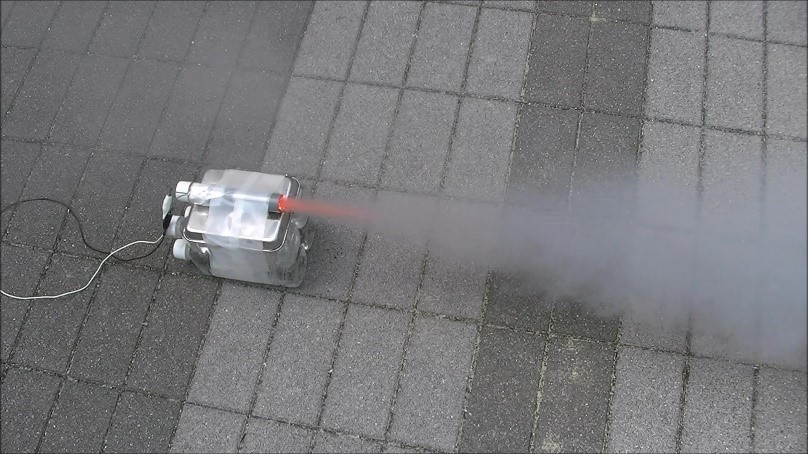
\includegraphics[height=3cm,clip]{okada/image/p_1.jpg}
  \caption{$P_1$試験}
  \label{fig:p1}
\end{figure}
\begin{figure}[H]
  \centering
  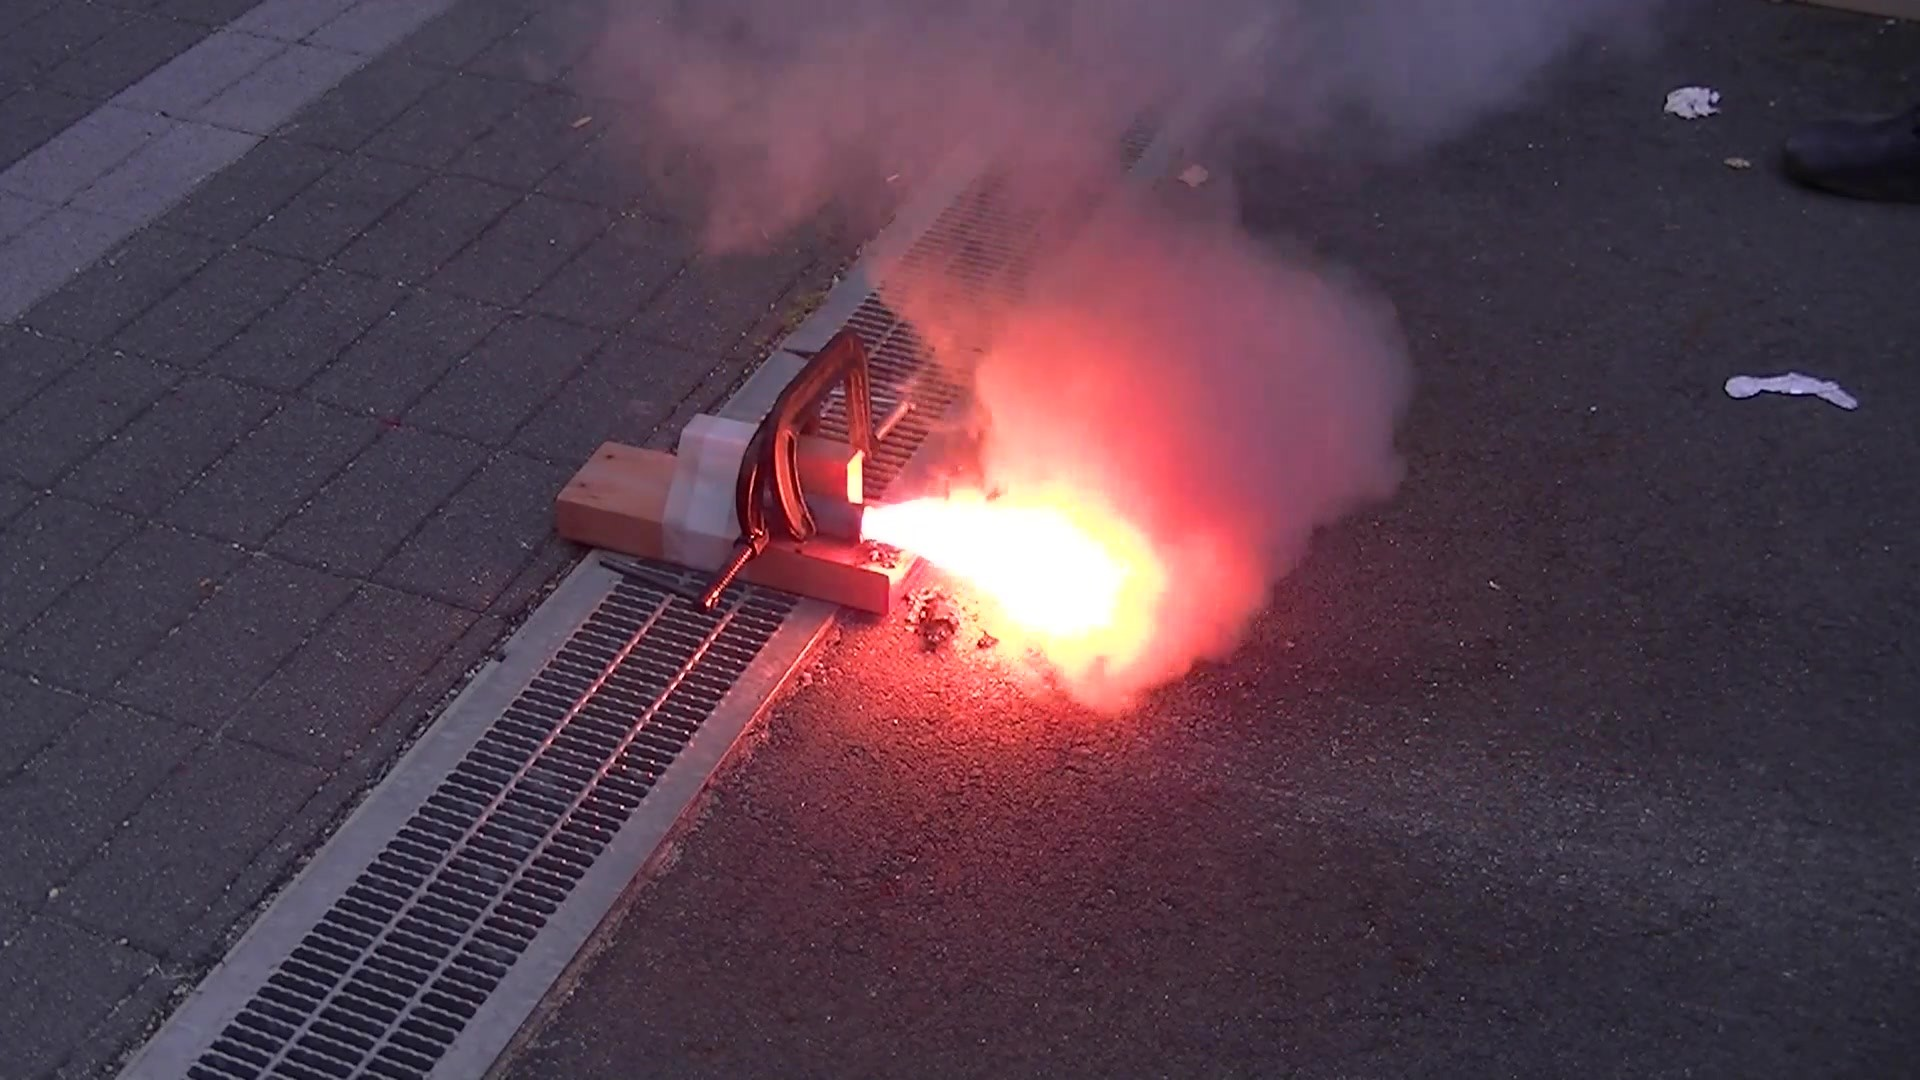
\includegraphics[height=3cm,clip]{okada/image/p_2.jpg}
  \caption{$P_2$試験}
  \label{fig:p2}
\end{figure}
\begin{figure}[H]
  \centering
  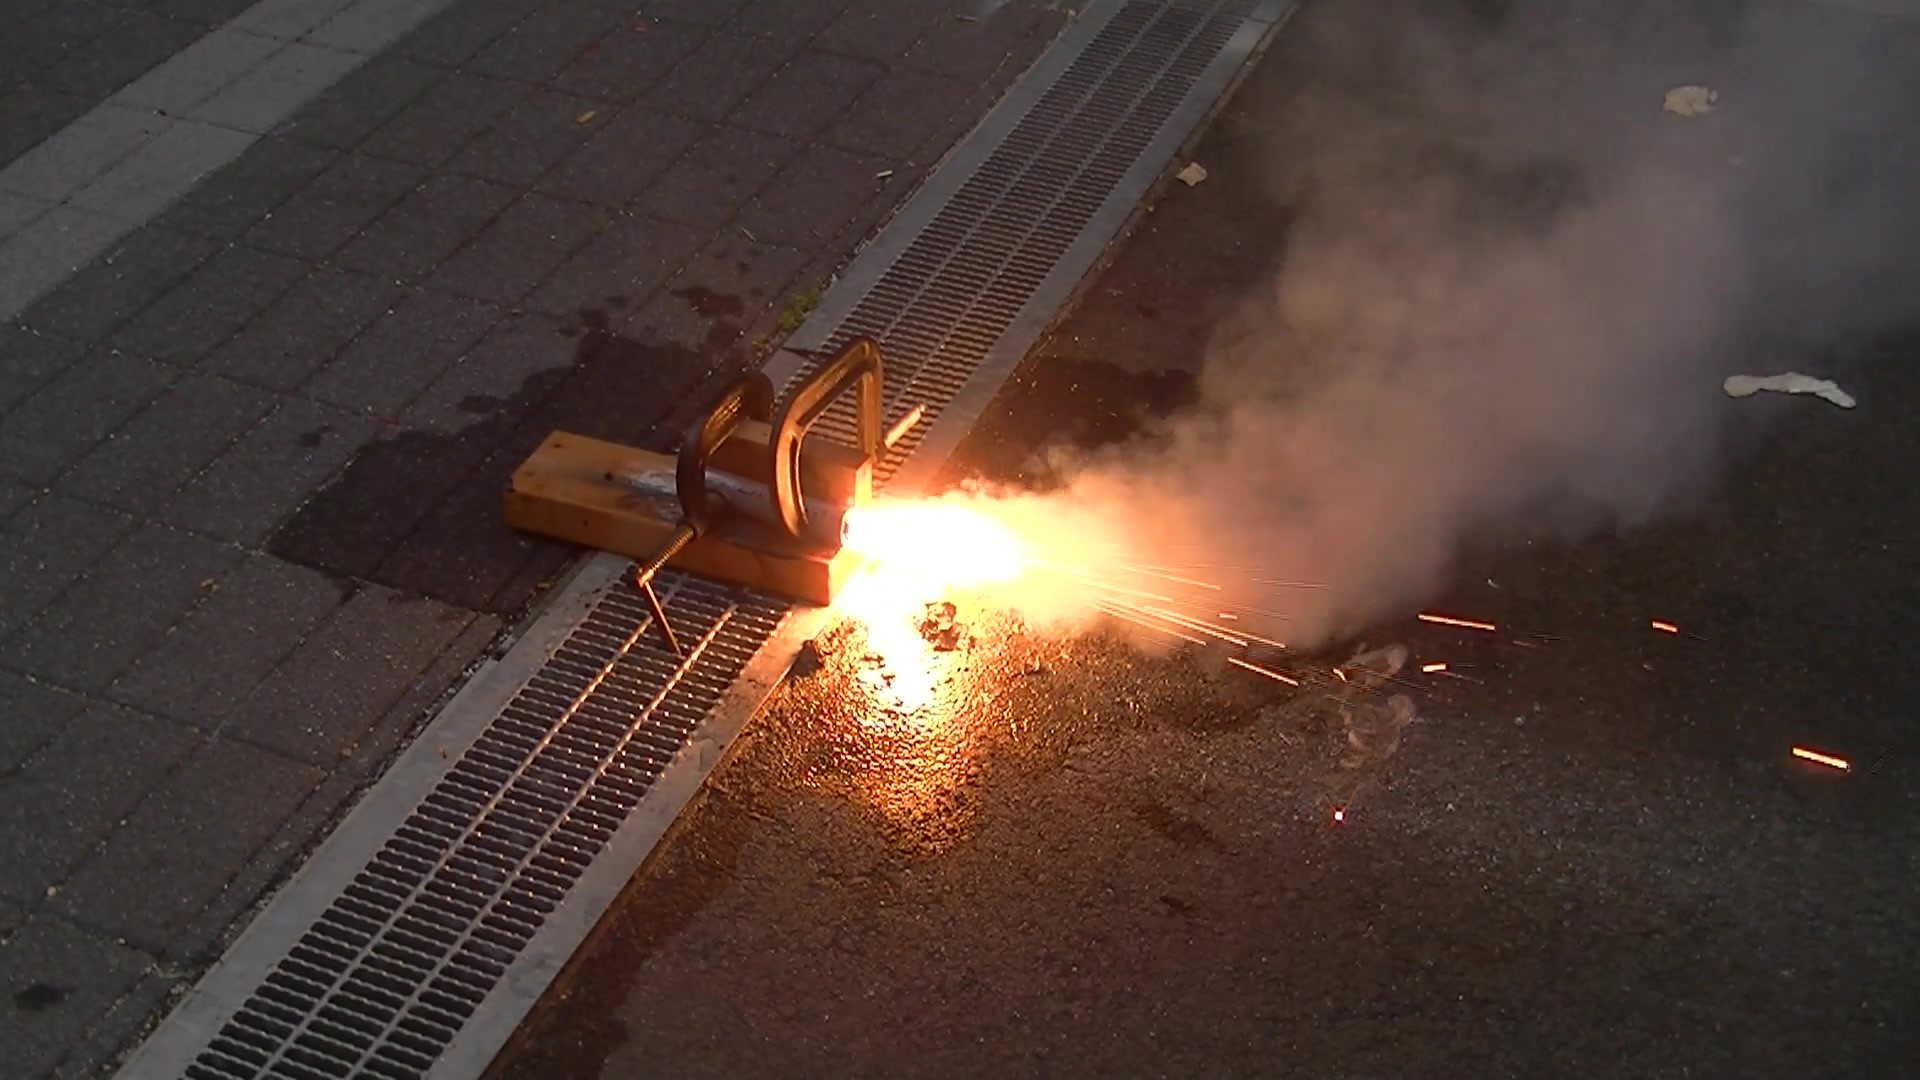
\includegraphics[height=3cm,clip]{okada/image/p_3.jpg}
  \caption{$P_3$試験}
  \label{fig:p3}
\end{figure}
$P_1$については問題なく安定して推進剤としての役割を果たしたが、$P_2$はただゆっくりと花火の様に燃焼しているだけであった。$P_3$は強力な推進剤となっていたが燃焼が不安定であった。
\subsection{試験結果の考察}
硝酸カリウムは酸素供給源であり、混ぜ合わせることで瞬間的に燃焼させることが出来る。噴射口は一つであるため、かかる圧力はすべて噴射口へと導かれ推進力が得られるとこういうことであろう。運動量保存則を考えれば良い。
 P2, P3の両試験において容器が溶けてしまったがこれはアルミ粉末を混ぜたことによって激しい反応を起こし、高温になったためと考えられる。対策として塩ビパイプよりも丈夫な容器を使えばよいだろう。

\section{ 【余談】 ロケット事件・大陸間弾道弾の実例と考察}
\subsection{中核派によるテロ事件から}
日本国内で無誘導弾の事件といえば革命的共産主義者同盟・中核派によるテロ事件が浮かび上がる。無誘導弾というよりは迫撃砲に近い。
 中核派のロケットは推進剤をロケットに詰め込んで発射させるのではなく黒色火薬を発射筒にセットして点火、発射させていたようである。
昔の火縄銃と同じで火薬を詰め込み、弾丸を込め、火をつけて発射するという大変古典的な方法を用いている。飛距離は2kmから4kmと結構な距離を記録しており、ただ単に火薬量が多かったからかロケットの形状がきっちりと計算されていたのかのどちらかが考えられる。複数の資料を見るにおそらく形状が良かったものと推測される。[4]
このころ(昭和50,60年代)なら普通、理科の実験などで塩素酸塩系をベースに推進剤が作られていたが塩素酸塩系は暴発しやすいため度々事故が起こっていた。[5]これを考えれば黒色火薬の燃焼による発射は比較的安全である。また慣性的エネルギーのみの飛行なので飛行中のエンジンの火薬質量を考慮せずに済み諸計算は大変楽である。
 発射後の話であるが、発射は上手くいっているにも関わらず信管の設計が難しかったようでほとんどが不発となっている。信管などの詳しいことは別の紙面にて述べる。

\subsection{朝鮮の弾道弾の発射試験から}
今日の朝鮮の弾道弾の発射試験の成果は目覚ましいものがある。1990年の弾道弾発射試験から今日までの実験を見ていればそれは明らかである。また2015年1月のSLBMの発射から2016年8月24日のSLBM発射試験でもそれは表れている。
2016年8月25日の朝鮮中央放送でSLBM発射についてアナウンサーが『主体朝鮮の核攻撃能力を一大誇示した。敬愛する金正恩同志の指導の下に戦略潜水艦弾道弾水中発射が正常に行われた』と述べており今まで以上にその発言が真実味を帯びているのを実感し、恐怖した。朝鮮の古い言葉に千里馬というのがあるが今は万里馬という時代語が使われ「千里馬よりも遥かに速く駆けていく」の意味がある。今が正にそれである。専門家が予想していたよりも我々が予想していたよりも朝鮮は速くに核弾頭を搭載する弾道弾の試験を行っている。また建国記念日である2016年9月9日には小型核弾頭の実験が敢行され核戦争の勢いである。一体朝鮮はどこに向かって速く駆けているのか。
さて今回行われた弾道弾の水中発射であるが、以前とはどこが違うのか。それは液体燃料と固体燃料の違いにある。液体燃料は注入したそばから揮発していくためすぐに打ち上げなければならない。その点、固体燃料であればある程度保管が出来るため使い勝手が良い。よって世界のトレンドは今や固体燃料である。
共和国朝鮮はソ連のコピー品のものを使っていたため液体燃料がトレンドであったが、方針を転換したのか固体燃料に切り替えたようだ。そこが前回とは違う点である。
次に掲載する写真は2016年8月25日に放送された朝鮮中央放送の一場面である。一段目左から「SLBM北極星本体写真」、「飛行1」、「飛行2」である。[6]

\begin{figure}[H]
  \centering
  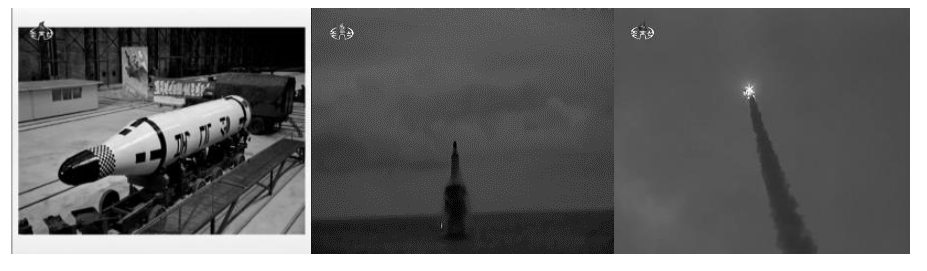
\includegraphics[height=3cm,clip]{okada/image/9no.png}
  \caption{本体写真、発射写真}
  \label{fig:9no}
\end{figure}

\newpage
\section*{参考文献}
\begin{enumerate}
  \item	火薬取締法及び航空法
  \item 佐々宏一著,「火薬工学」(森北出版, 2013年, p.3)
  \item JASON SMILEY, “EASY PVC ROCKETS”, 2005
  \item 複数セクトによる事件の被害及び犯行使用物の詳細資料(昭和60年~61年)
  \item 高等学校における火薬類の実験について(通産省, 昭和55年)
  \item \url{http://www.dprktoday.com/} (2016年8月25日配信の動画)
\end{enumerate}


\section{付録A 自家製ロケットエンジン高度計算手順}
ロケットの全重量:M(kg)\\

ロケットの直径:A($m^2$)=$\pi r^2$\\

空気抵抗力:$0.5\rm{Rho}\rm{Cd}\rm{A}v^2$\\
 Rho(空気の密度)=1.2($kg/m^3$)\\
 Cd(空気抵抗)=0.75(平均的な空気抵抗)\\
 まだ速度はわからないので速度を含めず計算する。これをkとする。\\

燃焼時間:$t=1/T$(sec)\\

重力加速度:$Mg=9.8M$\\

$q,x$の2つの値を次の様に定義する。\\
$q=\sqrt{[T-Mg]/k}$ Tは平均推力\\
$x=2kq/M$\\

完全燃焼速度:$v=q\frac{1-\exp{-xt}}{ 1+\exp{-xt}}$\\

動力飛行:$yb=\frac{-M}{2k}\ln \frac{T-Mg-kv^2} {T-M*g}$\\
慣性飛行:$yc=\frac{+M}{2k}\ln \frac{Mg+kv^2} {Mg}$\\

$yb+yc=Total\ Altitude$

\section{付録B 亜鉛と硫黄の混合火薬}
 粉末状の亜鉛と硫黄を混合し、点火すると激しく燃焼する。そのため高価な硝酸カリと粉糖による固体燃料の代替品、強化版として効果が期待できる。今回、亜鉛と硫黄の混合比率を変えてどのような挙動をするか観察することにした。
以下亜鉛をZ、硫黄をSと呼称する。
○条件○
次の3つに条件をわけて実験する。
\begin{itemize}
\item Z:50%、S:50%
\item Z:70%、S:30%
\item Z:80%、S:20%
\end{itemize}
\begin{figure}[H]
  \centering
  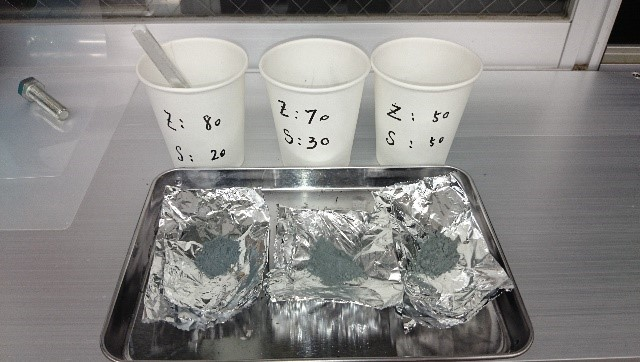
\includegraphics[height=4cm,clip]{okada/image/B.jpg}
  \caption{左からZ:80%, 70%, 50%}
  \label{fig:B}
\end{figure}
点火薬は黒色火薬(但、木炭の代りに粉糖を使用)1g程度を使用する。
\begin{itemize}
\item 手順
  \begin{itemize}
    \item 点火薬を使用せず点火、観察(各3g)
    \item 点火薬を使用して点火、観察(各3g)
    \item 3種を混合して点火、観察(各1g)
  \end{itemize}
\item 結果\\
この混合火薬は鈍感であり、点火薬がない場合ほとんど燃焼しない。亜鉛と硫黄のデータシートからわかるようにそれぞれ融解温度は500℃、400℃以上である。よってきっかけ(この場合は点火薬の黒色火薬)を与えてやればしっかりと燃焼する。
点火薬を使用した場合、Z,S50%はゆるやかに燃焼した。Z,S70%30%は燃焼が速かった(安定?)。Z,S80%20%はZ,S70%30%よりも燃焼速度が速く爆発的であった。これより、Zが増加するにつれ燃焼速度は増す傾向にあるのがわかる。
全てを混合した場合、まったく燃焼しなかった。混合比率はしっかりと計量する必要がある。
\end{itemize}
\begin{figure}[H]
  \centering
  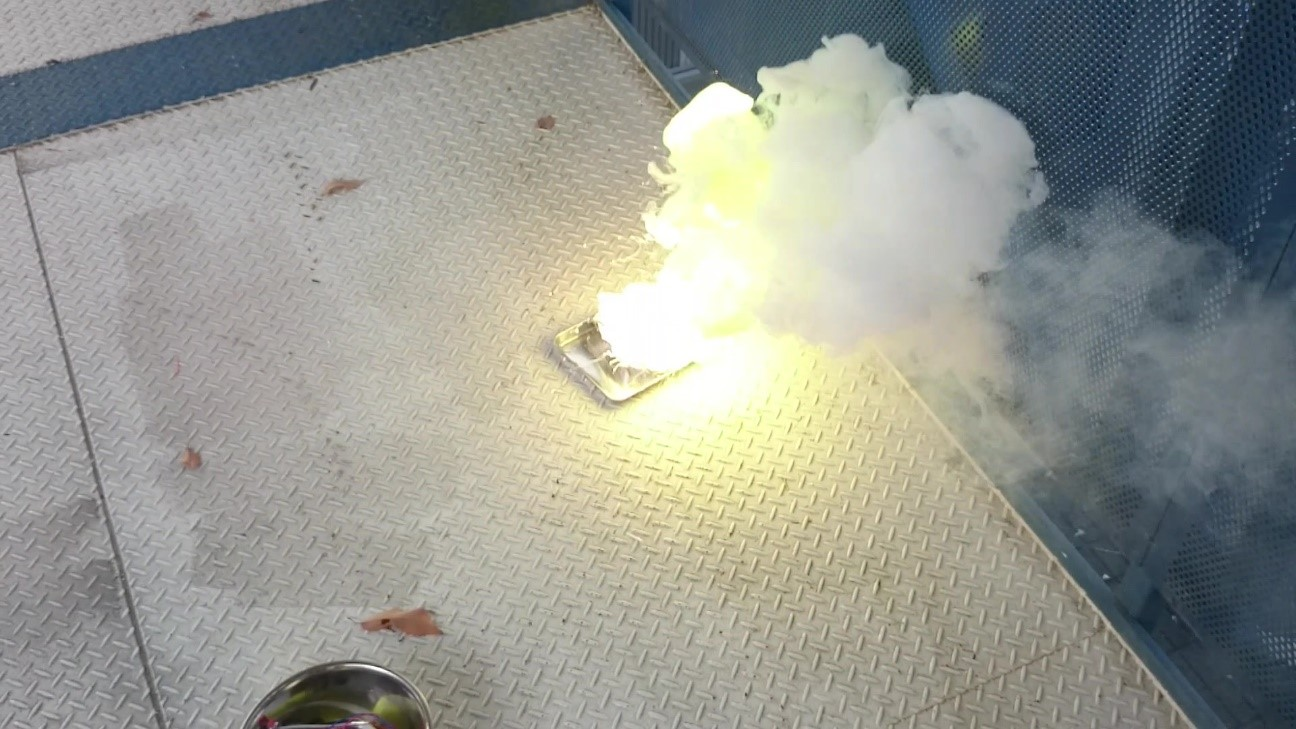
\includegraphics[height=4cm,clip]{okada/image/B_2.jpg}
  \caption{Z,S80%20%の燃焼}
  \label{fig:B}
\end{figure}

以上を踏まえると混合比率はZ > Sでなければ硝酸カリと粉糖の代替品にはならないことが理解できる。
亜鉛は500gで約1,500円と少々高いが硝酸カリウムは100gで約1,500円であるため固体燃料を制作するのであればコストの面から考えれば(制御面での難しさを除いて)、亜鉛と硫黄の混合火薬を使用するのが最善であろう。
